\documentclass[a4paper, 10pt]{article}
\usepackage{amsmath}
\usepackage{fancyhdr}
\usepackage{float}
\usepackage[a4paper, left=1in, right=1in, top=1in, bottom=1in]{geometry} % Adjust margins
\usepackage{graphicx}
\usepackage{listings}
\usepackage{matlab-prettifier}

\pagestyle{fancy}

\title{ECE 340 Lab 3}
\author{Omar Mahmoud\\1753607\\Section D21}
\date{10/22/2024}

\lhead{Omar Mahmoud}
\rhead{ECE 340 Lab 3}
\headheight 15pt

\begin{document}

%% Cover Page
\thispagestyle{empty}
\vfill
\maketitle
\vfill

\newpage

% Q1: Z-Transform
\section{Z-Transform}
A causal linear filter has the impulse response given by:
\begin{equation}
  h[n] = n(0.5)^n\sin(\frac{\pi n}{6})u[n]
\end{equation}
To get the impulse response $h_1[n]$ for $0\leq n\leq 10$ the following MATLAB script was used:
\begin{lstlisting}[style=Matlab-editor, basicstyle=\small\ttfamily]
  figure(1);

  % Plot the impulse response h_1[n]
  n = 0:10;
  h1 = n .* (0.5).^n .* sin((pi .* n)/6);
  stem(n, h1, 'LineWidth', 1, 'Color', 'r');
  title('Plot of h_1[n] for 0 \leq n \leq 10.');
  xlabel('n');
  ylabel('h_1[n]');
\end{lstlisting}
After running the script the following output was produced:
\begin{figure}[H]
  \centering
  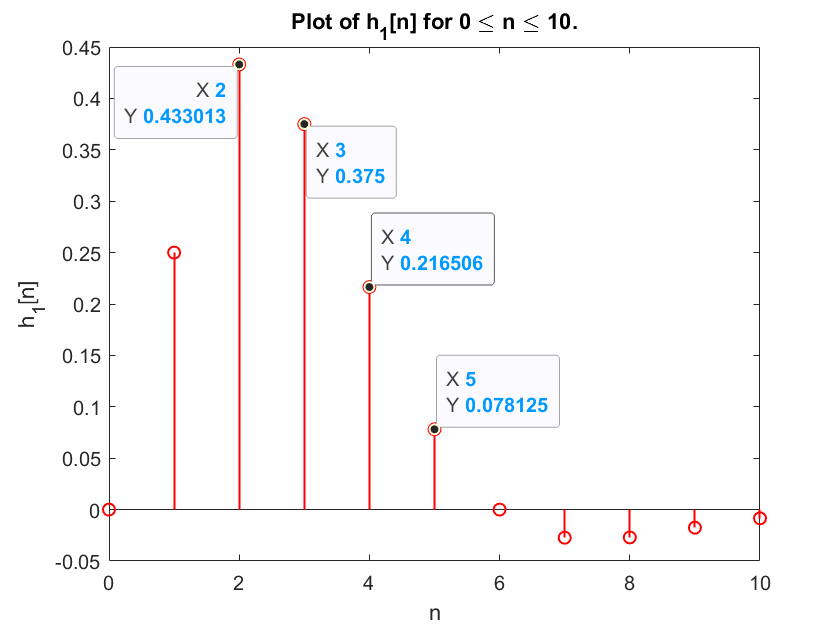
\includegraphics[width=10cm]{images/q1_a.png}
  \caption{Plot of $h_1[n]$ for $0\leq n\leq 10$.}
\end{figure}

\hfill

\noindent Using the $\mathcal{Z}$-Transform pair:
\begin{equation}
  \mathcal{Z}\{a^n\sin(\omega_0n)u[n]\} = \frac {az^{-1}\sin(\omega_0)} {1-2az^{-1}\cos(\omega_0)+a^2z^{-2}},
  \text{ ROC: } |z|>|a|
\end{equation} 
and the property:
\begin{equation}
  \mathcal{Z}\{nx[n]\} = -z\frac {dX(z)} {dz}
\end{equation}
the $H(z)$ of the system was determined through the following calculations:
\begin{center}
  $\mathcal{Z}\{h[n]\} = \mathcal{Z}\{n(0.5)^n\sin(\frac{\pi n}{6})u[n]\}$\\
  $H(e^{j\omega})= -z\frac{d}{dz}\mathcal{Z}\{(0.5)^n\sin(\frac{\pi n}{6})u[n]\}$\\
  $= -z\frac{d}{dz}(\frac {(0.5)z^{-1}\sin(\pi/6)} {1-2(0.5)z^{-1}\cos(\pi/6)+(0.5)^2z^{-2}})$\\
  $= \frac {4z^{-1}-z^{-3}} {16 - 16\sqrt{3}z^{-1}+20z^{-2}-4\sqrt{3}z^{-3}+z^{-4}}$
\end{center}

\hfill 

\noindent To get the impulse response of $H(z)$, $h_2[n]$ for $0\leq n\leq 10$ the following script is used: 
\begin{lstlisting}[style=Matlab-editor, basicstyle=\small\ttfamily]
  figure(2);

  % Get the frequency response of H(z) h2_[n]
  N = [0 4 0 -1];
  D = [16 -16*sqrt(3) 20 -4*sqrt(3) 1];
  
  x = zeros(1, 11);
  x(1) = 1; % Creates the impulse response
  
  h2 = filter(N, D, x);
  stem(n, h2, 'LineWidth' , 1, 'Color', 'b');
  title('Plot of Impulse Reponse, h_2[n], of H(z) for 0 \leq n \leq 10.');
  xlabel('n');
  ylabel('h_2[n]');
\end{lstlisting}
\begin{figure}[H]
  \centering
  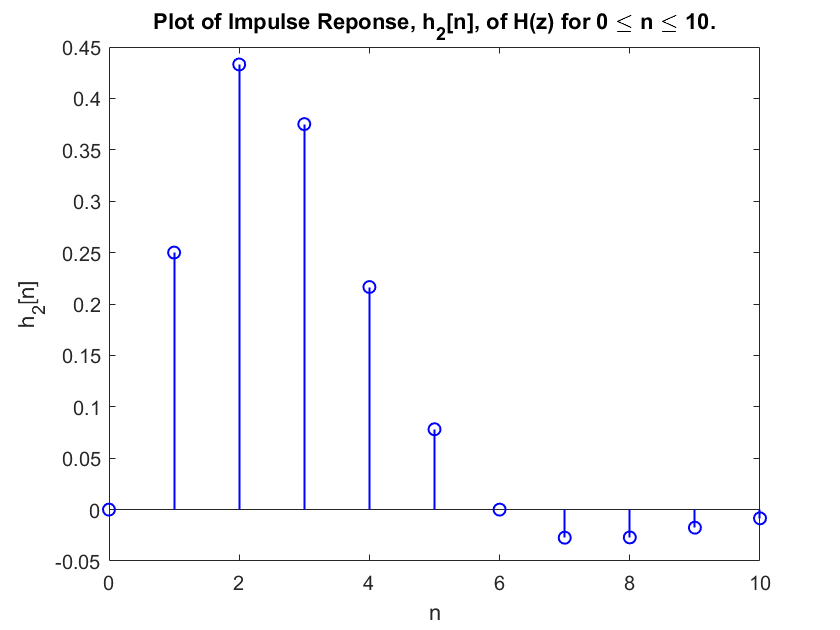
\includegraphics[width=10cm]{images/q1_c.png}
  \caption{Plot of Impulse Reponse, $h_2[n]$, of $H(z)$ for $0\leq n\leq 10$.}
\end{figure}

\hfill

\noindent To compare $h_1[n]$ and $h_2[n]$ on the same figure, the following script was ran:
\begin{lstlisting}[style=Matlab-editor, basicstyle=\small\ttfamily]
  figure(3);

  % Compare h_1[n] and h_2[n] on the same figure
  stem(n, h1, 'LineWidth', 1, 'Color', 'r');
  hold on;
  stem(n, h2, 'LineWidth' , 1, 'Color', 'b', 'LineStyle', '--');
  title('Plot of h_1[n] and h_2[n] for 0 \leq n \leq 10.');
  xlabel('n');
  ylabel('h_1[n] and h_2[n]');
  legend('h_1[n]', 'h_2[n]');
\end{lstlisting}
\begin{figure}[H]
  \centering
  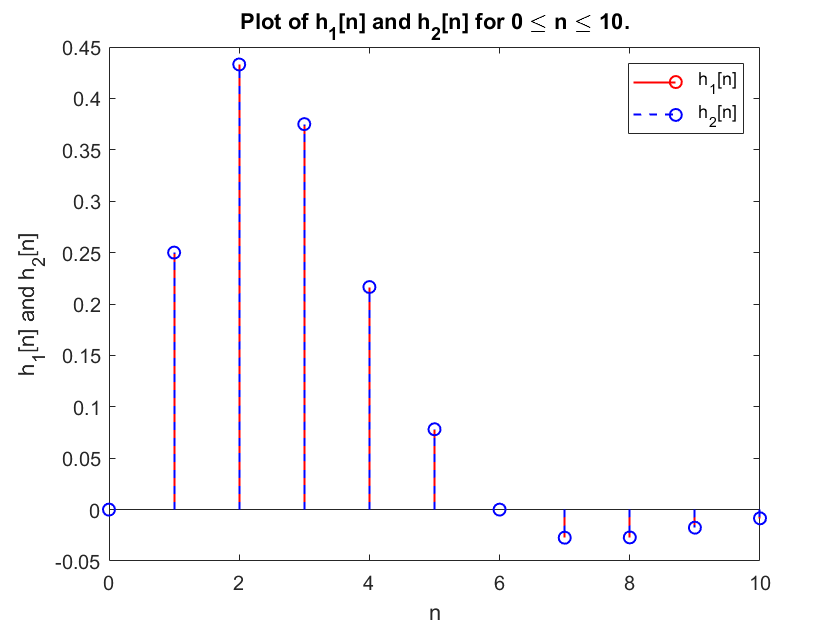
\includegraphics[width=10cm]{images/q1_d.png}
  \caption{Plot of $h_1[n]$ (solid red lines) and $h_2[n]$ (dotted blue lines) $0\leq n\leq 10$.}
\end{figure}
It is evident from the plot above that $h_2[n]$ is identical to $h_1[n]$. This shows that the filtered function is 
the same as the orginal signal, confirming our calculations for $H(z)$.

% Q1: Inverse Z-Transform & Pole-Zero Diagrams
\section{Inverse Z-Transform \& Pole-Zero Diagrams}
Given the transfer functions for two causal LTI systems:
\begin{equation}
  H_1(z) = \frac {2+2z^{-1}} {1-1.25z^{-1}}
\end{equation}
\begin{equation}
  H_2(z) = \frac {2+2z^{-1}} {1-0.8z^{-1}}
\end{equation}
Their plot-zero diagrams can be plotted using the following MATLAB script:
\begin{lstlisting}[style=Matlab-editor, basicstyle=\small\ttfamily]
  figure(1);

  % Plot pole-zero diagram for H1(z)
  subplot(2, 1, 1);
  N1 = [2 2];
  D1 = [1 -1.25];
  [z1, p1] = tf2zpk(N1, D1);
  
  zplane(z1, p1);
  title('Pole-Zero Diagram of H_1(z).');
  xlabel('Re{H_1(z)}');
  ylabel('Im{H_1(z)}');
  
  % Plot pole-zero diagram for H1(z)
  subplot(2, 1, 2);
  N2 = [2 2];
  D2 = [1 -0.8];
  [z2, p2] = tf2zpk(N2, D2);
  
  zplane(z2, p2);
  title('Pole-Zero Diagram of H_2(z).');
  xlabel('Re{H_2(z)}');
  ylabel('Im{H_2(z)}');
\end{lstlisting}
\begin{figure}[H]
  \centering
  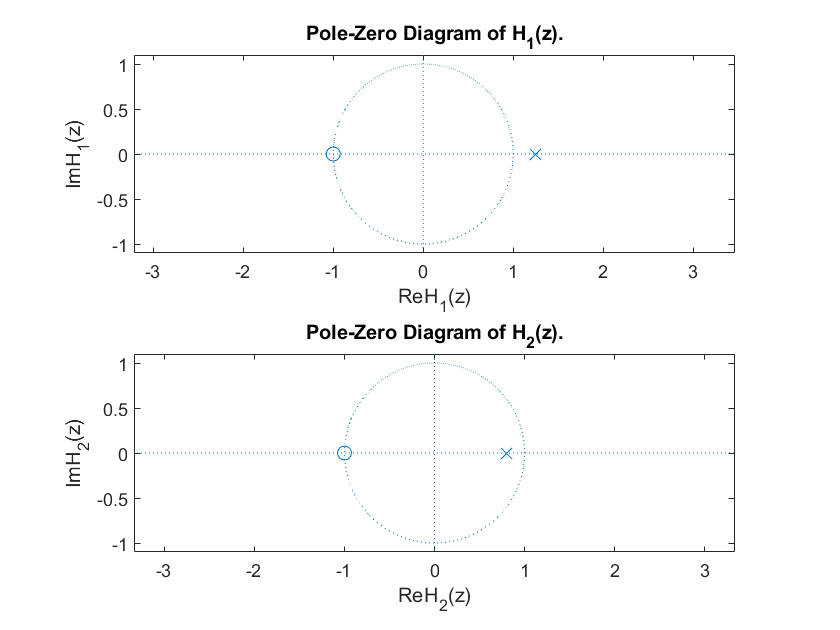
\includegraphics[width=12cm]{images/q2_a.png}
  \caption{Pole-Zero diagrams of $H_1(z)$ (top) and $H_2(z)$ (bottom).}
\end{figure}
From the plots above, it is clear that $H_1(z)$ has a pole outside of the ROC (region of convergence). This 
indicates that $H_1(z)$ is not BIBO stable. While for $H_2(z)$ it's pole is inside the ROC indicating that is it 
is BIBO stable.

\hfill

\noindent To plot the magnitude and phase of the frequency responses of the two systems in range $0\leq\omega\leq2\pi$,
the following script was used:
\begin{lstlisting}[style=Matlab-editor, basicstyle=\small\ttfamily]
  figure(2);

  % Plot the magnitude and phase of H1(z)
  [H1, w1] = freqz(N1, D1, 'whole');
  mag_H1 = abs(H1);
  phase_H1 = angle(H1);

  subplot(2, 2, 1);
  plot(w1/pi, mag_H1, 'LineWidth' , 1, 'Color', 'r');
  title('Plot of |H_1(z)|.');
  xlabel('\omega');
  ylabel('|H_1(z)|');

  subplot(2, 2, 2);
  plot(w1/pi, phase_H1, 'LineWidth' , 1, 'Color', 'r');
  title('Plot of \angle H_1(z).');
  xlabel('\omega');
  ylabel('\angle H_1(z)');

  % Plot the magnitude and phase of H2(z)
  [H2, w2] = freqz(N2, D2, 'whole');
  mag_H2 = abs(H2);
  phase_H2 = angle(H2);

  subplot(2, 2, 3);
  plot(w2/pi, mag_H2, 'LineWidth' , 1, 'Color', 'b');
  title('Plot of |H_2(z)|.');
  xlabel('\omega');
  ylabel('|H_2(z)|');

  subplot(2, 2, 4);
  plot(w2/pi, phase_H2, 'LineWidth' , 1, 'Color', 'b');
  title('Plot of \angle H_1(z).');
  xlabel('\omega');
  ylabel('\angle H_2(z)');
\end{lstlisting}
\begin{figure}[H]
  \centering
  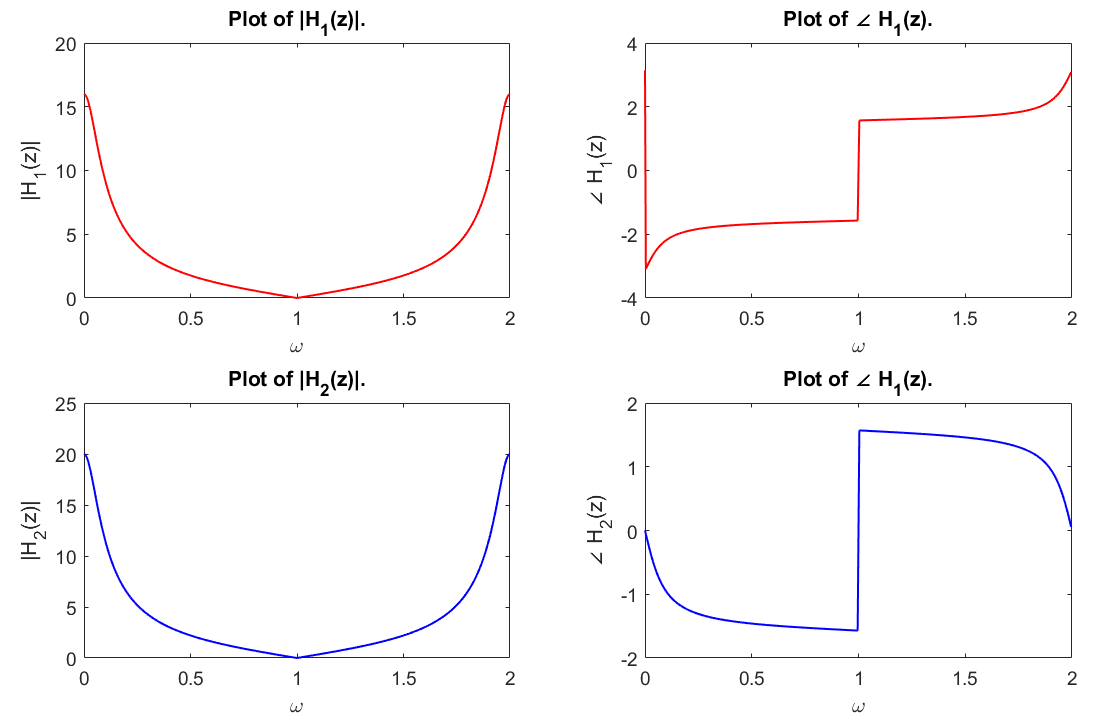
\includegraphics[width=14cm]{images/q2_b.png}
  \caption{Magnitude and phase plots of $H_1(z)$ (top) and $H_2(z)$.}
\end{figure}

\hfill

\noindent To obtain the impulse responses of the two systems $h_1[n]$ and $h_2[n]$ the transfer functions
were split and the inverse Z-transform of each part was taken:
\begin{equation}
  \begin{aligned}
    h_1[n] & = \mathcal{Z}\left\{\frac {2} {1-1.25z^{-1}}\right\} + \mathcal{Z}\left\{\frac {2z^{-1}} {1-1.25z^{-1}}\right\} \\
           & = 2(1.25)^nu[n]+2(1.25)^{n-1}u[n-1]
  \end{aligned}
\end{equation}
\begin{equation}
  \begin{aligned}
    h_1[n] & = \mathcal{Z}\left\{\frac {2} {1-0.8z^{-1}}\right\} + \mathcal{Z}\left\{\frac {2z^{-1}} {1-0.8z^{-1}}\right\} \\
           & = 2(0.8)^nu[n]+2(0.8)^{n-1}u[n-1]
  \end{aligned}
\end{equation}
To plot $h_1[n]$ and $h_2[n]$ for $0\leq n\leq 25$ in MATLAB the following script was ran:
\begin{lstlisting}[style=Matlab-editor, basicstyle=\small\ttfamily]
  figure(3);

  n = 0:25;
  u1_n = ones(1, 26); % u[n]
  u2_n = ones(1, 26); % u[n-1]
  u2_n(1) = 0;

  % Plot h1
  h1_n = (2.*(1.25).^n).*u1_n + (2.*(1.25).^(n-1)).*u2_n;
  subplot(2, 1, 1);
  stem(n, h1_n, 'LineWidth' , 1, 'Color', 'r');
  title('Plot of h_1[n].');
  xlabel('n');
  ylabel('h_1[n]');

  % Plot h2
  h2_n = (2.*(0.8).^n).*u1_n + (2.*(0.8).^(n-1)).*u2_n;
  subplot(2, 1, 2);
  stem(n, h2_n, 'LineWidth' , 1, 'Color', 'b');
  title('Plot of h_2[n].');
  xlabel('n');
  ylabel('h_2[n]');
\end{lstlisting}
\begin{figure}[H]
  \centering
  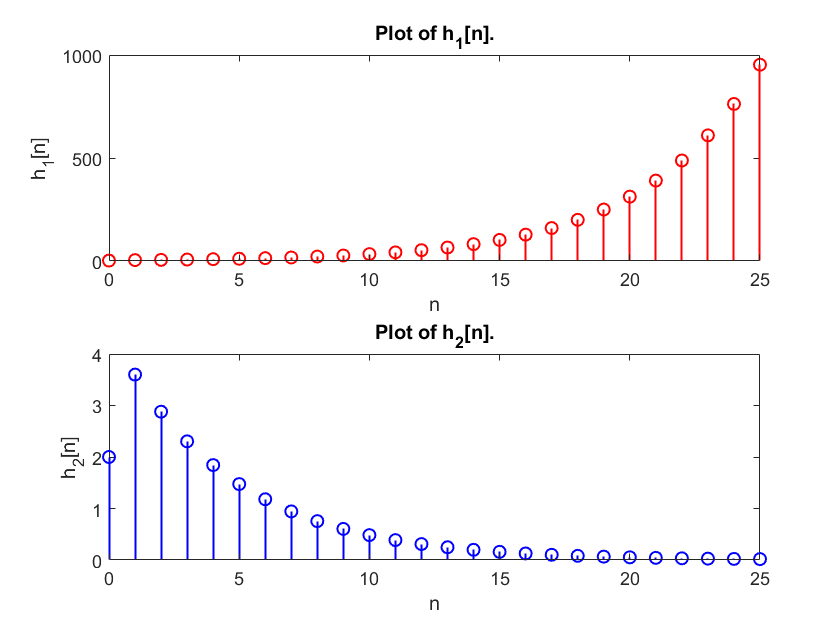
\includegraphics[width=10cm]{images/q2_c.png}
  \caption{Plots of $h1[n]$ (top) and $h_2[n]$ (bottom).}
\end{figure}
Previously, based on the plot-zero diagrams of $H_1(z)$ and $H_2(z)$ the conclusion was made that
$H_1(z)$ was not BIBO stable while $H_2(z)$ was. Seeing the plots above, it is evident that $h_1[n]$ is
exponentially growing, which means it will continue to approach infinity and the output will not be bound
when subjected to a bound input signal, hence it is not BIBO stable. On the other hand $h_2[n]$ displays exponential
decay approaching zero, hence it is BIBO stable. This data supports both conclusions made earlier.
\end{document}

